% This is "sig-alternate.tex" V2.1 April 2013
% This file should be compiled with V2.5 of "sig-alternate.cls" May 2012
%
% This example file demonstrates the use of the 'sig-alternate.cls'
% V2.5 LaTeX2e document class file. It is for those submitting
% articles to ACM Conference Proceedings WHO DO NOT WISH TO
% STRICTLY ADHERE TO THE SIGS (PUBS-BOARD-ENDORSED) STYLE.
% The 'sig-alternate.cls' file will produce a similar-looking,
% albeit, 'tighter' paper resulting in, invariably, fewer pages.
%
% ----------------------------------------------------------------------------------------------------------------
% This .tex file (and associated .cls V2.5) produces:
%       1) The Permission Statement
%       2) The Conference (location) Info information
%       3) The Copyright Line with ACM data
%       4) NO page numbers
%
% as against the acm_proc_article-sp.cls file which
% DOES NOT produce 1) thru' 3) above.
%
% Using 'sig-alternate.cls' you have control, however, from within
% the source .tex file, over both the CopyrightYear
% (defaulted to 200X) and the ACM Copyright Data
% (defaulted to X-XXXXX-XX-X/XX/XX).
% e.g.
% \CopyrightYear{2007} will cause 2007 to appear in the copyright line.
% \crdata{0-12345-67-8/90/12} will cause 0-12345-67-8/90/12 to appear in the copyright line.
%
% ---------------------------------------------------------------------------------------------------------------
% This .tex source is an example which *does* use
% the .bib file (from which the .bbl file % is produced).
% REMEMBER HOWEVER: After having produced the .bbl file,
% and prior to final submission, you *NEED* to 'insert'
% your .bbl file into your source .tex file so as to provide
% ONE 'self-contained' source file.
%
% ================= IF YOU HAVE QUESTIONS =======================
% Questions regarding the SIGS styles, SIGS policies and
% procedures, Conferences etc. should be sent to
% Adrienne Griscti (griscti@acm.org)
%
% Technical questions _only_ to
% Gerald Murray (murray@hq.acm.org)
% ===============================================================
%
% For tracking purposes - this is V2.0 - May 2012

\documentclass{sig-alternate}


\begin{document}

% Copyright
\setcopyright{acmcopyright}
%\setcopyright{acmlicensed}
%\setcopyright{rightsretained}
%\setcopyright{usgov}
%\setcopyright{usgovmixed}
%\setcopyright{cagov}
%\setcopyright{cagovmixed}


% DOI
\doi{}

% ISBN
\isbn{}

%Conference
\conferenceinfo{SIGCSE '17}{March 16--19, 2017, Seattle, WA, USA}

\acmPrice{\$15.00}

%
% --- Author Metadata here ---
\conferenceinfo{SIGCSE}{'17 Seattle, Washington USA}
%\CopyrightYear{2007} % Allows default copyright year (20XX) to be over-ridden - IF NEED BE.
%\crdata{0-12345-67-8/90/01}  % Allows default copyright data (0-89791-88-6/97/05) to be over-ridden - IF NEED BE.
% --- End of Author Metadata ---

\title{Playing with CORGIS: Diverse, Real-world Datasets for Introductory Computing}
%
% You need the command \numberofauthors to handle the 'placement
% and alignment' of the authors beneath the title.
%
% For aesthetic reasons, we recommend 'three authors at a time'
% i.e. three 'name/affiliation blocks' be placed beneath the title.
%
% NOTE: You are NOT restricted in how many 'rows' of
% "name/affiliations" may appear. We just ask that you restrict
% the number of 'columns' to three.
%
% Because of the available 'opening page real-estate'
% we ask you to refrain from putting more than six authors
% (two rows with three columns) beneath the article title.
% More than six makes the first-page appear very cluttered indeed.
%
% Use the \alignauthor commands to handle the names
% and affiliations for an 'aesthetic maximum' of six authors.
% Add names, affiliations, addresses for
% the seventh etc. author(s) as the argument for the
% \additionalauthors command.
% These 'additional authors' will be output/set for you
% without further effort on your part as the last section in
% the body of your article BEFORE References or any Appendices.

\numberofauthors{5} %  in this sample file, there are a *total*
% of EIGHT authors. SIX appear on the 'first-page' (for formatting
% reasons) and the remaining two appear in the \additionalauthors section.
%
\author{
% You can go ahead and credit any number of authors here,
% e.g. one 'row of three' or two rows (consisting of one row of three
% and a second row of one, two or three).
%
% The command \alignauthor (no curly braces needed) should
% precede each author name, affiliation/snail-mail address and
% e-mail address. Additionally, tag each line of
% affiliation/address with \affaddr, and tag the
% e-mail address with \email.
%
% 1st. author
\alignauthor
Anonymous\\
       \affaddr{Anonymous}\\
       \affaddr{Anonymous}\\
       \affaddr{Anonymous}\\
       \email{Anonymous}
% 2nd. author
}

\date{1 September 2016}
% Just remember to make sure that the TOTAL number of authors
% is the number that will appear on the first page PLUS the
% number that will appear in the \additionalauthors section.

\maketitle
\begin{abstract}
Abstract goes here
\end{abstract}


%
% The code below should be generated by the tool at
% http://dl.acm.org/ccs.cfm
% Please copy and paste the code instead of the example below. 
%
\begin{CCSXML}
<ccs2012>
<concept>
<concept_id>10002951.10002952.10003219</concept_id>
<concept_desc>Information systems~Information integration</concept_desc>
<concept_significance>500</concept_significance>
</concept>
<concept>
<concept_id>10002951.10002952</concept_id>
<concept_desc>Information systems~Data management systems</concept_desc>
<concept_significance>100</concept_significance>
</concept>
<concept>
<concept_id>10003456.10003457.10003527.10003528</concept_id>
<concept_desc>Social and professional topics~Computational thinking</concept_desc>
<concept_significance>300</concept_significance>
</concept>
<concept>
<concept_id>10003456.10003457.10003527.10003530</concept_id>
<concept_desc>Social and professional topics~Model curricula</concept_desc>
<concept_significance>300</concept_significance>
</concept>
<concept>
<concept_id>10003456.10003457.10003527.10003539</concept_id>
<concept_desc>Social and professional topics~Computing literacy</concept_desc>
<concept_significance>100</concept_significance>
</concept>
</ccs2012>
\end{CCSXML}

\ccsdesc[500]{Information systems~Information integration}
\ccsdesc[100]{Information systems~Data management systems}
\ccsdesc[300]{Social and professional topics~Computational thinking}
\ccsdesc[300]{Social and professional topics~Model curricula}
\ccsdesc[100]{Social and professional topics~Computing literacy}



%
% End generated code
%

%
%  Use this command to print the description
%
\printccsdesc

\keywords{corgis; data; data science; pedagogy; motivation; microworld; real-world; authentic; big data}

\section{Introduction}

\section{Theory}

A data science microworld

\subsection{Abstraction}

Students must understand the relationship between the process of \textit{abstracting} and \textit{interpreting} data.
In the context of this project, we describe Abstraction as the process of simplifying and representing real-world phenomenon using concrete, computable properties.
The process of abstraction necessarily throws away context and data that is not practical for solving problems of an expected stakeholder.

\subsection{Educational Theory}

Situated Learning Theory suggests that authentic contexts are crucial for students.

\section{Related and Prior Work}

\subsection{RealTimeWeb}

The RealTimeWeb made it easy for instructors to bring 

\subsection{BRIDGES}

\subsection{Framework for Social Good}

\section{Design}

\begin{figure}[h]
    \centering
    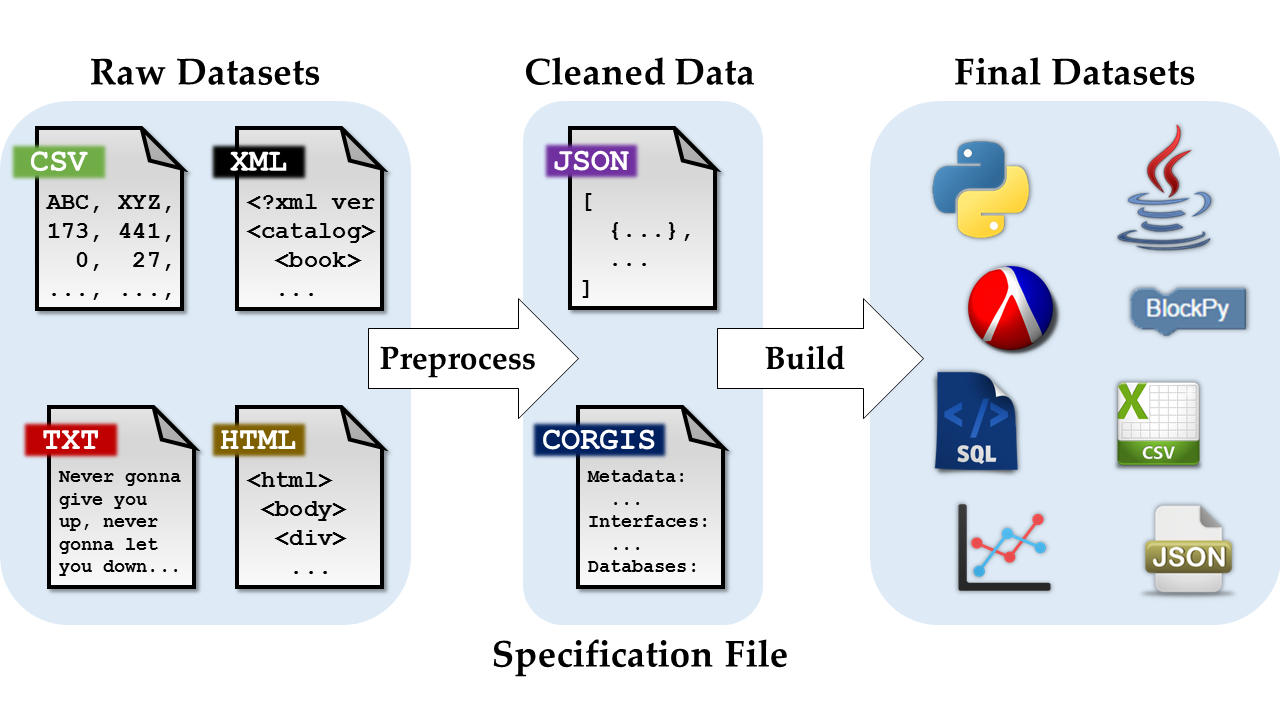
\includegraphics[width=.5\textwidth]{graphics/process}
    \caption{The CORGIS Build Process}
    \label{fig:corgis-build}
\end{figure}

\subsection{Finding Datasets}

The major goal was to have multiple datasets that could satisfy every major career path that potential students could be seeking.

We draw on data from open-access sources, including governments, research publications, journalists, non-profits, and industry.

For simplicity's sake, we only use datasets that are publicly licensed, so that students do not have to sign Non-disclosure agreements.

\subsection{Dataset Preparation}

Every dataset tends to require some level of cleaning, which can be an ad-hoc process.

The prepared dataset is expected to have certain pedagogical and conventional attributes, meant to simplify students' access and facilitate manipulation of the dataset.

Pedagogical attributes

Splicing in datasets


\subsection{Specification Files}

The CORGIS Specification files are a YAML-based file format that defines metadata, interfaces, and structure of the dataset that is external to the data itself.

Comments for individual fields of the data are specified through JSON Paths.

\subsection{Bindings}

\subsubsection{Python}

%import crime
%crime.get_all()
%crime.by_state('Delaware')

\subsubsection{Java}

The Java version of the library 

\subsubsection{Racket}
\subsubsection{BlockPy}
\subsubsection{Visualizer}
\subsubsection{SQL}
\subsubsection{CSV and JSON}

\subsection{Gallery}

Every dataset is associated with a list of tags to help students search.

\begin{figure}[h]
    \centering
    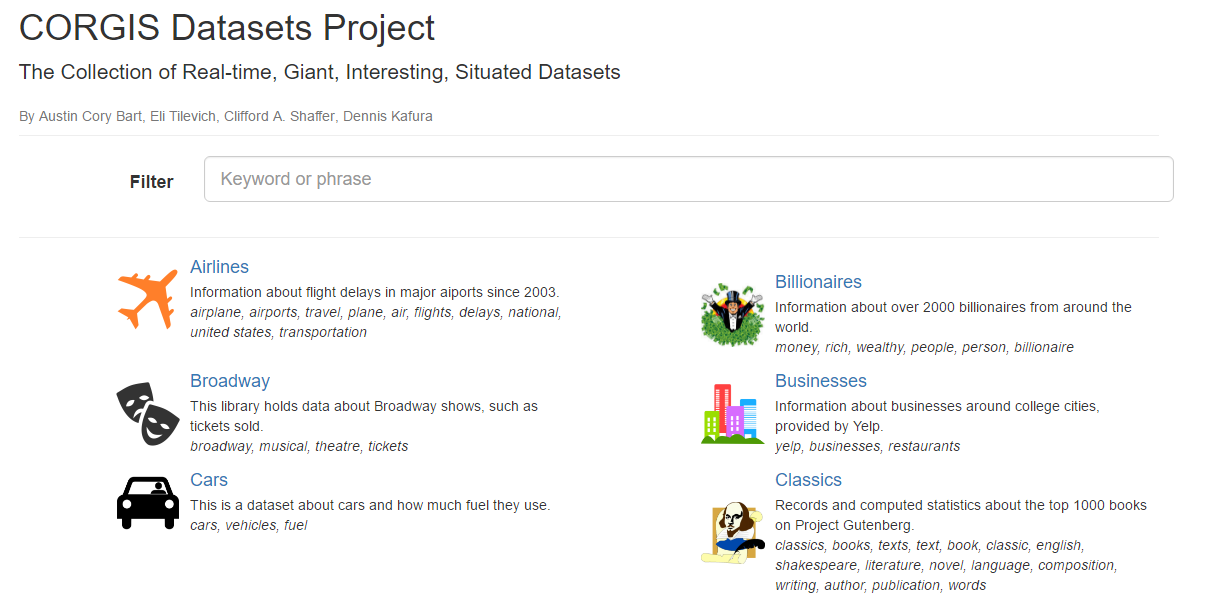
\includegraphics[width=.5\textwidth]{graphics/gallery}
    \caption{The CORGIS Gallery}
    \label{fig:corgis-gallery}
\end{figure}

\section{Assignments}

The CORGIS project is built 

\subsection{Exploratory Analysis}

The Visualizer facilitates early discovery of the datasets before students even encounter the programming curriculum.

\subsection{Data Mapping}

The Explorer was designed to help students understand and navigate the structure of the datasets.

\subsection{Data Analysis}

Our vision was for professors to allow their students to choose from the complete collection of datasets.

Students can pick a dataset

An important component of our project is for students to describe the abstractions used in the project and the inherent limitations of the dataset.

\section{Evaluation}

\subsection{Metrics}

At the time of writing, there are N datasets in the CORGIS project, and we are actively working to expand this set.

\subsubsection{Structure}

The Average Branch Factor (ABF) is the mean number of fields in all objects of the structure.

The Height of the dataset is the maximal depth of the tree.

\subsubsection{Data}

\begin{figure}[hb!]
\centering
\begin{tabular}{l|lllll}
            & C & M & I & S & U  \\\hline
Abstraction & 15.9 & 26.9      & \textbf{39.1*}  & \textbf{39.4*}    & \textbf{50.1*} \\
Cohort      & 14.6 & 26.6      & 25.1   & 28.3      & 33.2  \\
Data        & 11.1 & 16.6       & 19.8    & 25.1     & 30.9  \\
Ethics      & 17.8 & 24.4      & 21.6   & \textbf{26.5*}    & \textbf{45.3*}  \\
Programs    & 16.3 & 29.5      & \textbf{27.8*}  & \textbf{38.5*}    & \textbf{71.1*}
\end{tabular}
\caption{Correlation between Students' Intent to Continue vs. Components of the Course with respect to Motivational Components (End of semester)}
\label{tbl-continue}
\end{figure}


Ideally, every dataset would have an equal ratio of every data type, so that students could experience.

In terms of raw elements, 

\begin{figure*}
\begin{tabular}{ l | c c | c c c c c c|}
 & \multicolumn{2}{|c|}{Structure} & \multicolumn{6}{|c|}{Data Types} \\
Name & ABF & Height & List & Object & Boolean & Integer & String & Float \\\hline
airlines & 3 & 4 & 1 & 8 & 0 & 18 & 5 & 0\\
billionaires & 4 & 4 & 1 & 6 & 4 & 4 & 12 & 2\\
broadway & 11 & 2 & 1 & 1 & 0 & 7 & 3 & 0\\
cars & 23 & 2 & 1 & 1 & 0 & 10 & 10 & 3\\
classics & 4 & 5 & 5 & 10 & 0 & 14 & 10 & 14\\
constructionpermits & 3 & 5 & 2 & 5 & 0 & 9 & 4 & 0\\
constructionspending & 12 & 4 & 1 & 10 & 0 & 51 & 2 & 0\\
drugbank & 9 & 5 & 7 & 3 & 0 & 0 & 18 & 2\\
drugs & 5 & 4 & 2 & 2 & 0 & 6 & 3 & 0\\
school & 3 & 6 & 6 & 15 & 0 & 24 & 2 & 7\\
energy & 8 & 4 & 1 & 6 & 0 & 1 & 0 & 43\\
finance & 61 & 5 & 2 & 4 & 0 & 240 & 1 & 0\\
grads & 21 & 2 & 1 & 1 & 0 & 17 & 2 & 2\\
health & 6 & 2 & 1 & 1 & 0 & 3 & 2 & 1\\
races & 3 & 6 & 21 & 82 & 0 & 40 & 79 & 87\\
immigration & 42 & 3 & 1 & 4 & 0 & 166 & 0 & 0\\
injuries & 3 & 3 & 1 & 5 & 0 & 3 & 8 & 3\\
labor & 2 & 6 & 1 & 73 & 0 & 11 & 39 & 39\\
medalofhonor & 3 & 4 & 1 & 8 & 1 & 7 & 12 & 2\\
music & 9 & 3 & 1 & 4 & 0 & 3 & 9 & 21\\
publishers & 6 & 3 & 1 & 4 & 11 & 3 & 1 & 6\\
realestate & 3 & 4 & 1 & 6 & 0 & 0 & 18 & 0\\
retailservices & 15 & 4 & 1 & 6 & 0 & 31 & 2 & 9\\
scripts & 4 & 5 & 4 & 4 & 0 & 3 & 11 & 1\\
skyscrapers & 6 & 4 & 1 & 7 & 25 & 10 & 5 & 1\\
slavery & 4 & 5 & 2 & 13 & 0 & 0 & 40 & 0\\
suicideattacks & 3 & 4 & 3 & 8 & 1 & 7 & 15 & 0\\
supremecourt & 3 & 5 & 1 & 29 & 7 & 36 & 43 & 0\\
tate & 3 & 4 & 1 & 7 & 0 & 4 & 11 & 3\\
\end{tabular}
    \caption{Metrics on CORGIS Datasets}
    \label{fig:corgis-metrics}
\end{figure*}

\subsection{Surveys}

4 students did not consent to their survey results, and 6 students chose not to complete the survey.
This yielded an 80\% response rate.

Table \ref{tbl-continue} reveals a fascinating connection between students' motivation with respect to the content and context and their long-term intent to continue in computing.

\subsection{Usage}

\subsubsection{Search Logs}

We collected log data over the course of a semester to 

\subsubsection{Final Project Usage}

Students were given freedom to select any dataset for their final project.

\section{Future Work}

Configurable Binding Settings

Advanced Data Science Tools
A major limitation of dataset preparation is the expertise required to clean and munge datasets into a format suitable for students.
Although there is significant dedicated research to lowering barriers for this process, it is still the work of a programmer with time and interest.
Further, every dataset demands some level of domain-knowledge to correctly and meaningfully arrange the fields.

Relational data

Artifical data

An open question in our research is how important the 

\section{Conclusions}


\section{Acknowledgments}


\section{References}

\thebibliography{}

\end{document}